% !TEX root = DesignDocument.tex

\chapter{Project Management}

\section{Team Member's Roles}
The team members for this project are Andrew Fagrey, Jayson Kjenstad, and Samantha Kranstz. The team members were selected by the Senior Design course instructor, Dr. McGough. All team members serve as developers and testers for each part of this project. The respective roles for each project are as follows:

\begin{itemize}
\item Andrew Fagrey acted as a type of scrum master as well as a developer on the project focusing mainly on the web application development.
\item Samantha Kranstz served as a developer on the project focusing mainly on the web API development.
\item Jayson Kjenstad served as a developer on the project focusing mainly on the tablet application development.
\end{itemize}

\section{Project  Management Approach}
We will be developing our project using the Agile development methodology. This will allow the team flexibility as we develop the product over the course of two semesters. Each sprint will be approximately two and a half weeks long. The project source code, product backlog, and documentation are hosted in a Bitbucket repository owned by Dr. McGough. The user stories, sprint milestones, and sprint issues are also managed in Bitbucket. The team makes use of the Bitbucket wiki pages that allow the team to post questions and have discussions about various aspects of the project.

\section{Stakeholder Information}
The stakeholders for this project include Dr. McGough, Dr. Karlsson, and Brian Butterfield. The team members are also stakeholders for the project. Future users of the product could also be considered stakeholders for the project if the development of the project continues after this senior design course.

\subsection{Customer or End User (Product Owner)}
The end users for this product will primarily be educational institutions. Professors and office personnel in educational institutions will be able to make use of the tablet application and web application, whereas students could make use of an accompanying student mobile application.

\subsection{Management or Instructor (Scrum Master)}
Andrew Fagrey acts as a mini scrum master for this project by helping to break up the work for each sprint and solve team development obstacles. Dr. Karlsson helps to manage the overall project, and Brian Butterfield helps with overall design and architecture of the project. 

\subsection{Investors}
There are currently no financial investors for this project. This could change if development continues after the Senior Design course.

\subsection{Developers and Testers}
The main developers for this project are Andrew Fagrey, Samantha Kranstz, and Jayson Kjenstad. All developers for this project will also be testers. Every developer who writes code will be responsible for writing the accompanying tests for that code. The project manager for this project is Dr. Karlsson. Brian Butterfield is the chief architect for this project.

\section{Budget}
This project doesn't really have a specific budget. None of the developers are receiving any financial compensation for working on this project. All of the tools that are being used in the development of the project are downloaded free of charge.\\

\noindent Microsoft Visual Studio Enterprise Edition and Microsoft Azure are being used free of charge due to 
educational discounts for each. Dr. Karlsson purchased a Samsung Galaxy Tablet for the team to use in the development of the tablet application. The purchase of the Samsung tablet has been the only cost to the team besides tuition.

\section{Intellectual Property and Licensing}
The South Dakota School of Mines and Technology and the South Dakota Board of Regents have intellectual property rights over this project.

\section{Sprint  Overview}
The DoorPanes project will be implemented in phases. They are as follows:

\subsection{User Stories and Requirements Gathering}
This phase will be used to collect all user stories, requirements, limitations, and specifications for the project from the respective clients. The software contract between the clients and the developers will be written and signed during this phase of the development as well.

\subsection{Researching and Designing}
During this phase, we will be researching our options for the design, software, and hardware that could be used in the development of the project. After exploring these options, we will be deciding on the best course of action to take in the development of the project.

\subsection{Application Development}
All application development will occur during this phase of the project. The implementation of this project will follow all of the client's requirements gathered in the earlier phases in the project.

\subsection{Prototype Development}
The result of our developmental efforts will be a prototype of the project. The prototype will be a basic proof of concept. It will not be a full-fledged example of how the product will work, but just enough of an implementation to showcase the possibilities if the project were completed. The prototype for the project will include a responsive web application, a web API with a few calendar event endpoints, and a tablet application. 

\subsection{Testing Phase}
After the initial development of the project, we will spend some time thoroughly testing the code that we have developed for the project and the prototypes.

\subsection{Delivery}
The final phase of the project will be the delivery of the product. This product includes several components: the web application, the web API, and the tablet application. 

\section{Terminology and Acronyms}
Below is a list of terms and acronyms that will be used throughout this design document to describe the various parts of the DoorPanes project.

\begin{itemize}
\item MVC - Model View Controller
\item VS - Microsoft Visual Studio
\item API - Application Programming Interface
\end{itemize}

\section{Sprint Schedule}
The sprint schedule is listed below. The sprint schedule was largely determined by the Senior Design course instructor.

\begin{itemize}
\item Sprint 1: 9/12/16 - 10/1/16
\item Sprint 2: 10/10/16 - 10/29/16
\item Sprint 3: 11/7/16 - 11/26/16
\item Sprint 4: 1/9/17 - 1/27/16
\item Sprint 5: 2/6/17 - 2/24/17
\item Sprint 6: 3/13/17 - 4/6/17
\item Design Fair: 4/25/17
\end{itemize}

\section{Timeline}
\begin{figure}[tbh]
\begin{center}
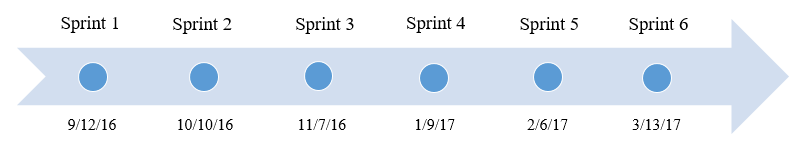
\includegraphics[width=0.75\textwidth]{./timeline.PNG}
\end{center}
\label{sprinttimeline}
\end{figure}

\section{Backlogs}

\subsection*{Sprint 1}
\begin{itemize}
	\item Set up Azure
	\item Create Azure database
	\item Create Azure app service
	\item Research Tablet vs Odroid Options
	\item Learn Xamarin\footnote{See Appendix \ref{XamarinAppendix} \label{note10}}
\end{itemize}

\subsection*{Sprint 2}
\begin{itemize}
\item Create Web App project
\item Upload Web App project to Azure
\item Create Web API project
\item Update Web API project to Azure
\item Create Xamarin tablet application with a login page\textsuperscript{\ref{note10}}
\item Create API endpoints for moving schedule data back and forth
\end{itemize}

\subsection*{Sprint 3}
\begin{itemize}
\item \#18 Tablet App - Android Kiosk Mode for Tablet App
\item \#24 Web API - Create Professor Model
\item \#25 Web API - Create Office Personnel Model
\item \#26 Web API - Create Calendar Event Model
\item \#27 Web API - Model Location
\item \#28 Web API - Create GetCalendarEvent endpoint
\item \#29 Web API - Create GetCalendarEvents endpoint
\item \#30 Web App - Open calendar framework JSON events
\item \#31 Web App - Connect calendar event creation to database
\item \#32 Web API - Create SaveCalendarEvents endpoint
\item \#33 Web App - Load events from database when navigating to dashboard controller
\item \#35 Create Unit test projects for both the web applications and web API projects
\item \#36 Tablet App - Create Calendar View
\item \#37 Web App (TEAM) - Create wireframe for design
\item \#38 Tablet App (TEAM) - Create wireframe for tablet app
\item \#39 Tablet App - Create communications class
\item \#40 Tablet App - Create a way to display JSON calendar events
\item \#41 Web API - Repository Layer
\item \#42 Tablet App - Move Tablet Code
\item \#43 Web API - Serialize data
\end{itemize}

\subsection*{Sprint 4}
\begin{itemize}
\item Create middleman project
\item \#53 Android calendar framework JSON function
\item \#54 Understand how event ownership works
\end{itemize}

\subsection*{Sprint 5}
\begin{itemize}
\item \#58 Web App - Add code to insert calendar events into database
\item \#59 Web App - Grab JSON from calendar framework
\item \#60 Web App - Load events from database
\item \#61 Web API - Fix Models
\item \#62 Web API - Create GetCalendarEventsByOwner endpoint
\item \#64 Web API - Create GetCalendarEventsByRoom
\item Tablet App - Create pop-up window with description
\item Tablet App - Modify week view class open source
\item Tablet App - Added synchronization button
\item Tablet App - Implement continuous synchronization
\item Tablet App - Create login page
\item Testing
\end{itemize}

\subsection*{Sprint 6}
\begin{itemize}
\item \#66 Web App - Add Authorization code
\item \#67 Web API - Display options endpoints
\item \#68 Web API - Create GetCalendarEventsByRange
\item \#69 Web API - Model updates
\item Web App - Create distinguished views for each type of user
\item Web App - Role based detection
\item Web App - Registration process
\item Web App - Database table integration and referencing
\item Web App - Repetition to generate repeated calendar events
\item Web App - Handle temporary canceled events
\item Tablet App - Add a view to select calendar based on faculty or room
\item Tablet App - Token authentication
\item Tablet App - GUI modifications
\item Tablet App - Handle temporary canceled events
\item Testing
\end{itemize}

\section{Burndown Charts}
\begin{figure}[tbh]
\begin{center}
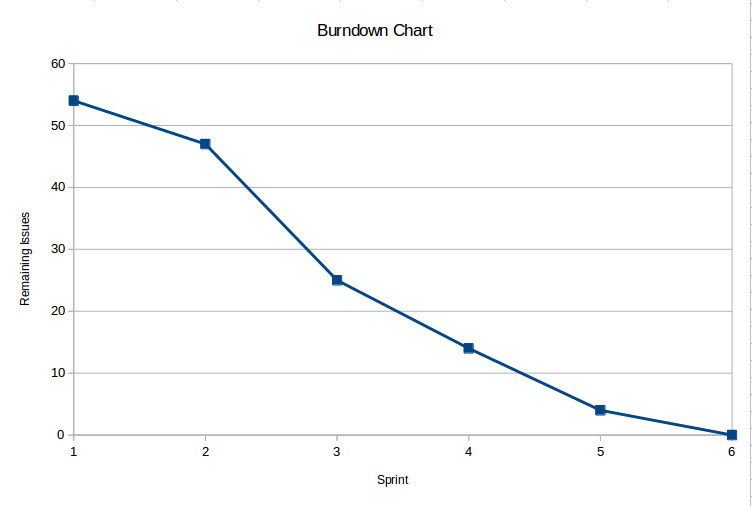
\includegraphics[width=0.75\textwidth]{./Burndown.png}
\end{center}
\label{BurndownChart}
\end{figure}

\section{Development Environment}
To setup a machine for development towards this project, the developer must ensure that his development machine meets the list of requirements shown below. Development machines must have:

\begin{itemize}
\item Windows 10 or later running on the machine.
\item Microsoft Visual Studio Enterprise Edition installed.
\item Android Studio installed.
\item Android SDK with a minimum API level of 23 installed.
\end{itemize}

\noindent The project files and code for the web application and web API must be downloaded from the Bitbucket repository. The web application and web API projects (as well as the testing projects for each) are contained in a Visual Studio Solution. Opening up the Visual Studio solution file should open the web application and web API projects, along with their respective testing projects.\\ 

\noindent The Android Studio solution is contained in a separate repository. The solution can be downloaded from the repository, and then it can be opened, built, and run in Android Studio.

\section{Development IDE and Tools}
Each team member is using their SDSM\&T Tablet PC running Microsoft Windows 10 for the development of this project. The team is using Microsoft Visual Studio Enterprise Edition as an IDE for this project for the web application and the web API. Microsoft Azure is being used as the back-end for this project. The Android tablet app is being developed with Android Studio and the Android SDK. We also are using a Samsung Galaxy Tab A8 for the tablet application development.

\section{Source  Control}
Bitbucket is used for code versioning and management. Dr. McGough created a repository and added each team member to the repository. All team members have write access. A second repository was created to host the tablet application source code. A developer can connect to the repository by responding to an invite from an administrator of the repository.

\section{Dependencies}
The web application and web API projects are dependent on the Microsoft ASP.NET platform, whereas the Android application will be depended on the Android SDK.

\section{Build  Environment}
The web application and web API projects are built and run in Visual Studio. The testing projects for the web application and web API are also built and run in Visual Studio. The Android application is built and run in Android Studio.

\section{Development Machine Setup}
A machine can be used for development on this project if it is capable of running Windows 10, Visual Studio, and Android Studio with the SDK. To setup your machine, follow the following steps:

\begin{itemize}
\item Make sure you are are running Windows 10. If not, you must either purchase Windows 10 and install it on your current machine, or upgrade to a machine capable of running Windows 10. 
\item Purchase and install Microsoft Visual Studio Enterprise Edition.
\item Download Android Studio.
\end{itemize}


